\begin{appendices}
\chapter{Bloch Vektörü}
\paragraph{}
Bu bölümde, Hamiltonyen matrisinden Bloch vektörü ve ilgili büyüklükler elde edilecektir. Bloch vektörü, iki seviyeli saf (pure) kuantum mekaniksel bir sistemin geometrik temsilini anlamamıza yardımcı olur. \emph{Bloch} ismi, Nobel ödüllü Felix Bloch'dan gelmektedir \cite{Bloch:1946zza}. Spin ve izospin gibi ikili kuantum mekaniksel sistemlerin analizi ve yoğunluk matrisinin davranışını anlamak için ortaya konan Bloch küresi ve Bloch vektörü, matematiksel özellikleri nedeniyle başka alanlarda da kullanılır. Biz, Hamiltonyen'in özdeğerlerini, özvektörlerini, ölçülebilirlerini ve özbaza döndüren açıyı bulmak için Bloch vektöründen yararlanacağız. Bloch vektör tanımı Hamiltonyen'den bağımsız herhangi bir $ 2 \times 2 $ sanal matris için de yazılabilir.
\begin{align}
\nonumber H_{\alpha\beta} &= \mqty(H_{ee} & H_{ex} \\ H_{xe} & H_{xx}) \text{ ,}\\
\nonumber				   &= \frac{H_{ee} + H_{xx}}{2} I + \frac{1}{2} \mqty(H_{ee} - H_{xx} & 2 H_{ex}\\ 2 H_{xe} & H_{xx}-H_{ee})  \text{ ,}\\
						   &= k I + \frac{1}{2} \vec{\sigma} \cdot \vec{B} \text{.}
\end{align}

Evrime katkı sağlamayan ve birim matrisle orantılı olan $ kI $ terimini ayrı yazdık. $ k $ katsayısı, Hamiltonyen matrisinin köşegen elemanlarının toplamının yarısıdır ve $ I $ matrisi ise $2$ boyutlu birim matristir. Denklemde $ \vec{\sigma} $ Pauli-spin matris vektörüdür. $ \vec{B} $ ise \emph{Bloch vektörüdür} ve aşağıdaki gibi tanımlanır.
\begin{equation}\label{eqn:appBloch_B_Hmat}
    \vec{B} = \mqty(H_{ex} & 0 & [H_{ee}-H_{xx}]/2 ) \text{ .}
\end{equation}

Bloch vektörü kullanılarak özdeğerler ve özvektörler kolayca yazılabilir. Özdeğerler aşağıdaki gibidir.
\begin{align} \label{eqn:appBloch_B_Ozdeg}
    \lambda_{1} = k + \abs{\vec{B}} \text{ ,}\\
    \lambda_{2} = k - \abs{\vec{B}} \text{ .}
\end{align}
Bu özdeğerlere karşılık gelen özvektörler de Bloch vektörünün elemanları cinsinden yazılabilir.
\begin{align}
    \vec{v}_{1} =& \mqty(B_{x} - iB_{y} \\ \abs{\vec{B}} - B_{z}) \text{ ,}\\
    \vec{v}_{2} =& \mqty(B_{x} - iB_{y} \\ -\abs{\vec{B}} - B_{z}) \text{ .}
\end{align}

Bloch vektörleri yardımıyla sistemin geometrik gösterimi yapılabilir. İlgilendiğimiz sistemlerde Hamiltonyen gerçel (reel) olduğundan dolayı Bloch vektörünün $ y $ bileşeni sıfırdır. Bu da $ \vec{B} $ vektörünü $ x-z $ düzlemine iz düşürür. 
\begin{figure}[!hbt]
	\centering
    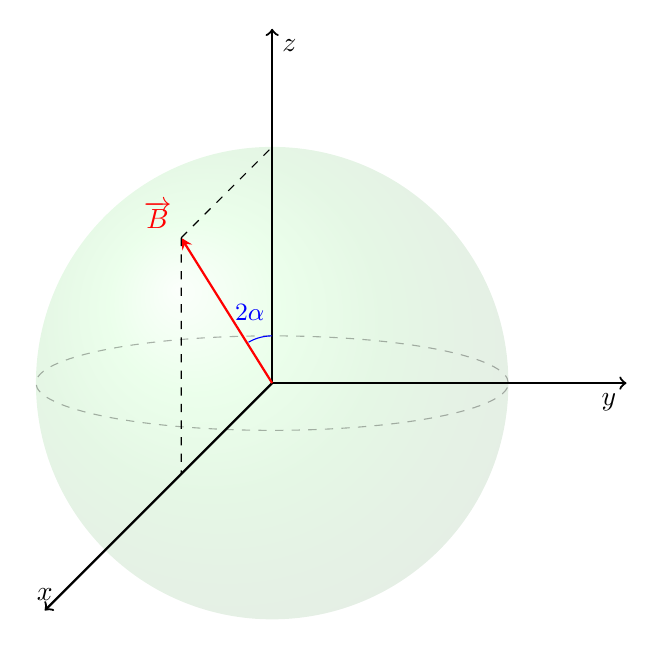
\begin{tikzpicture}[font = \sansmath, scale=1.5]
\coordinate (O) at (0,0,0);
\coordinate (B) at (0,2,2);

% ball background color
\shade[ball color = green, opacity = 0.1] (0,0) circle [radius = 2cm];

% Coordinate System
\draw[thick,->] (0,0,0) -- (3,0,0) node[anchor=north east]{$y$};
\draw[thick,->] (0,0,0) -- (0,3,0) node[anchor=north west]{$z$};
\draw[thick,->] (0,0,0) -- (0,0,5) node[anchor=south]{$x$};

% ellipse at center
\draw[dashed, color=black, opacity = 0.3] (0,0) ellipse ({2} and {0.4});

%draw a vector from origin to point (P) 
\draw[thick,-stealth,color=red] (O) -- (B);

%draw projection on xy plane, and a connecting line
\draw[dashed, color=black] (B) -- (0,0,2);
\draw[dashed, color=black] (B) -- (0,2,0);

% Text
\node[anchor=south east, color=red] at (0,2,2) {$\overrightarrow{B} $};

%draw theta arc and label, using rotated coordinate system
\draw[color = blue] (0cm,0.4cm) arc (90:120:0.4cm);
% Text
\node[anchor=south, color=blue] at (0,0.6,0.4) {$$\small $2\alpha$ $$};
  
\end{tikzpicture}
    \caption[Bloch Küresi ve Bloch Vektörü]{Bloch Küresi ve Bloch Vektörü}
    \label{fig:blochVec}%
\end{figure}

Nötrino salınımlarında, bir bazdan diğer baza geçerken dönme matrisleri $ \mathcal{R}_{\theta} $ kullanılır. Bloch vektörü $ \vec{B} $ ile $ z $-ekseni arasında açı karışım açısının iki katı olarak tanımlanır. Bu tanım altında Bloch vektörünün bileşenleri $ B_{x} = \abs{\vec{B}}\sin 2\alpha $, $ B_{y}=0 $ ve $ B_{z} = \abs{\vec{B}} \cos 2\alpha $ şeklinde yazılır. Özvektörler de karışım açısı $ \alpha $ cinsinden yazılabilir. Boşluk salınımları ile karşılaştırdığımızda $ \alpha $ açısı ile $ \theta $ açısı eş değerdir.
\begin{align} \label{eqn:appBloch_B_Ozvec}
    \vec{v}_{1} =& 2 \abs{\vec{B}} \sin \alpha \mqty(\cos \alpha \\ \sin \alpha) \text{ ,}\\
    \vec{v}_{2} =& 2 \abs{\vec{B}} \cos \alpha -\mqty(\sin \alpha \\-\cos \alpha) \text{ .}
\end{align}
Özvektörlerin başındaki katsayı, normalizasyon katsayısıdır.

\eqref{eqn:appBloch_B_Hmat} numaralı denklem, matris notasyonu kullanılarak elde edilmiştir. Benzer işlemleri ve denklemleri Hamiltonyen operatörünün bileşenleri için de yazabiliriz.
\begin{equation} \label{eqn:appBloch_B}
    \vec{B} = \mqty(\mel{\nu_{e}}{\hat{H}}{\nu_{x}} & 0 & (\mel{\nu_{e}}{\hat{H}}{\nu_{e}} - \mel{\nu_{x}}{\hat{H}}{\nu_{x}})/2  ) \text{ .}
\end{equation}

Bloch vektörü, Hamiltonyen'in hangi bazda yazıldığına göre değişir \cite{Pehlivan:2011hp}. \eqref{eqn:appBloch_B} numaralı denklemde çeşni bazı kullanılarak yazılmıştır. Bloch vektörünün $ z $-ekseni ile arasındaki açı $ 2\alpha $ ise aşağıdaki gibi belirlenir.
\begin{equation} \label{eqn:appBloch_mixAng}
\cos 2\alpha = \frac{B_{z}}{\abs{\vec{B}}} \text{ ,} \qquad \sin 2\alpha = \frac{B_{x}}{\abs{\vec{B}}} \text{ .}
\end{equation}

Elde edilen açıların işareti, analitik düzlemde hangi kuadrantta olduğunu belirler. Uygun trigonometrik özdeşlikler ile istenilen kuadranta geçiş yapılır. 

\end{appendices}